\section{Problem Statement}
Aggregate, coordinated motion of bodies, such as a flock of birds, school of fish or herd of animals commonly occurs in nature (Figure~\ref{fig:intro}). Creating such flocking behavior in simulation is also a well-studied problem in computer graphics. In a SIGGRAPH paper in 1987~\cite{cr-siggraph}, Craig Reynolds first defined the term ``boid flocking" to refer to such flocking behavior, where ``boid" refers to each independent actor that works in coordination with others to produce the overall flocking effect. His work~\cite{cr-siggraph} also produced a behavioral model and physics-based simulation of such flocking. In this 

\begin{figure}[ht!]
\centering
    \begin{subfigure}[t]{0.45\textwidth}
        \centering
        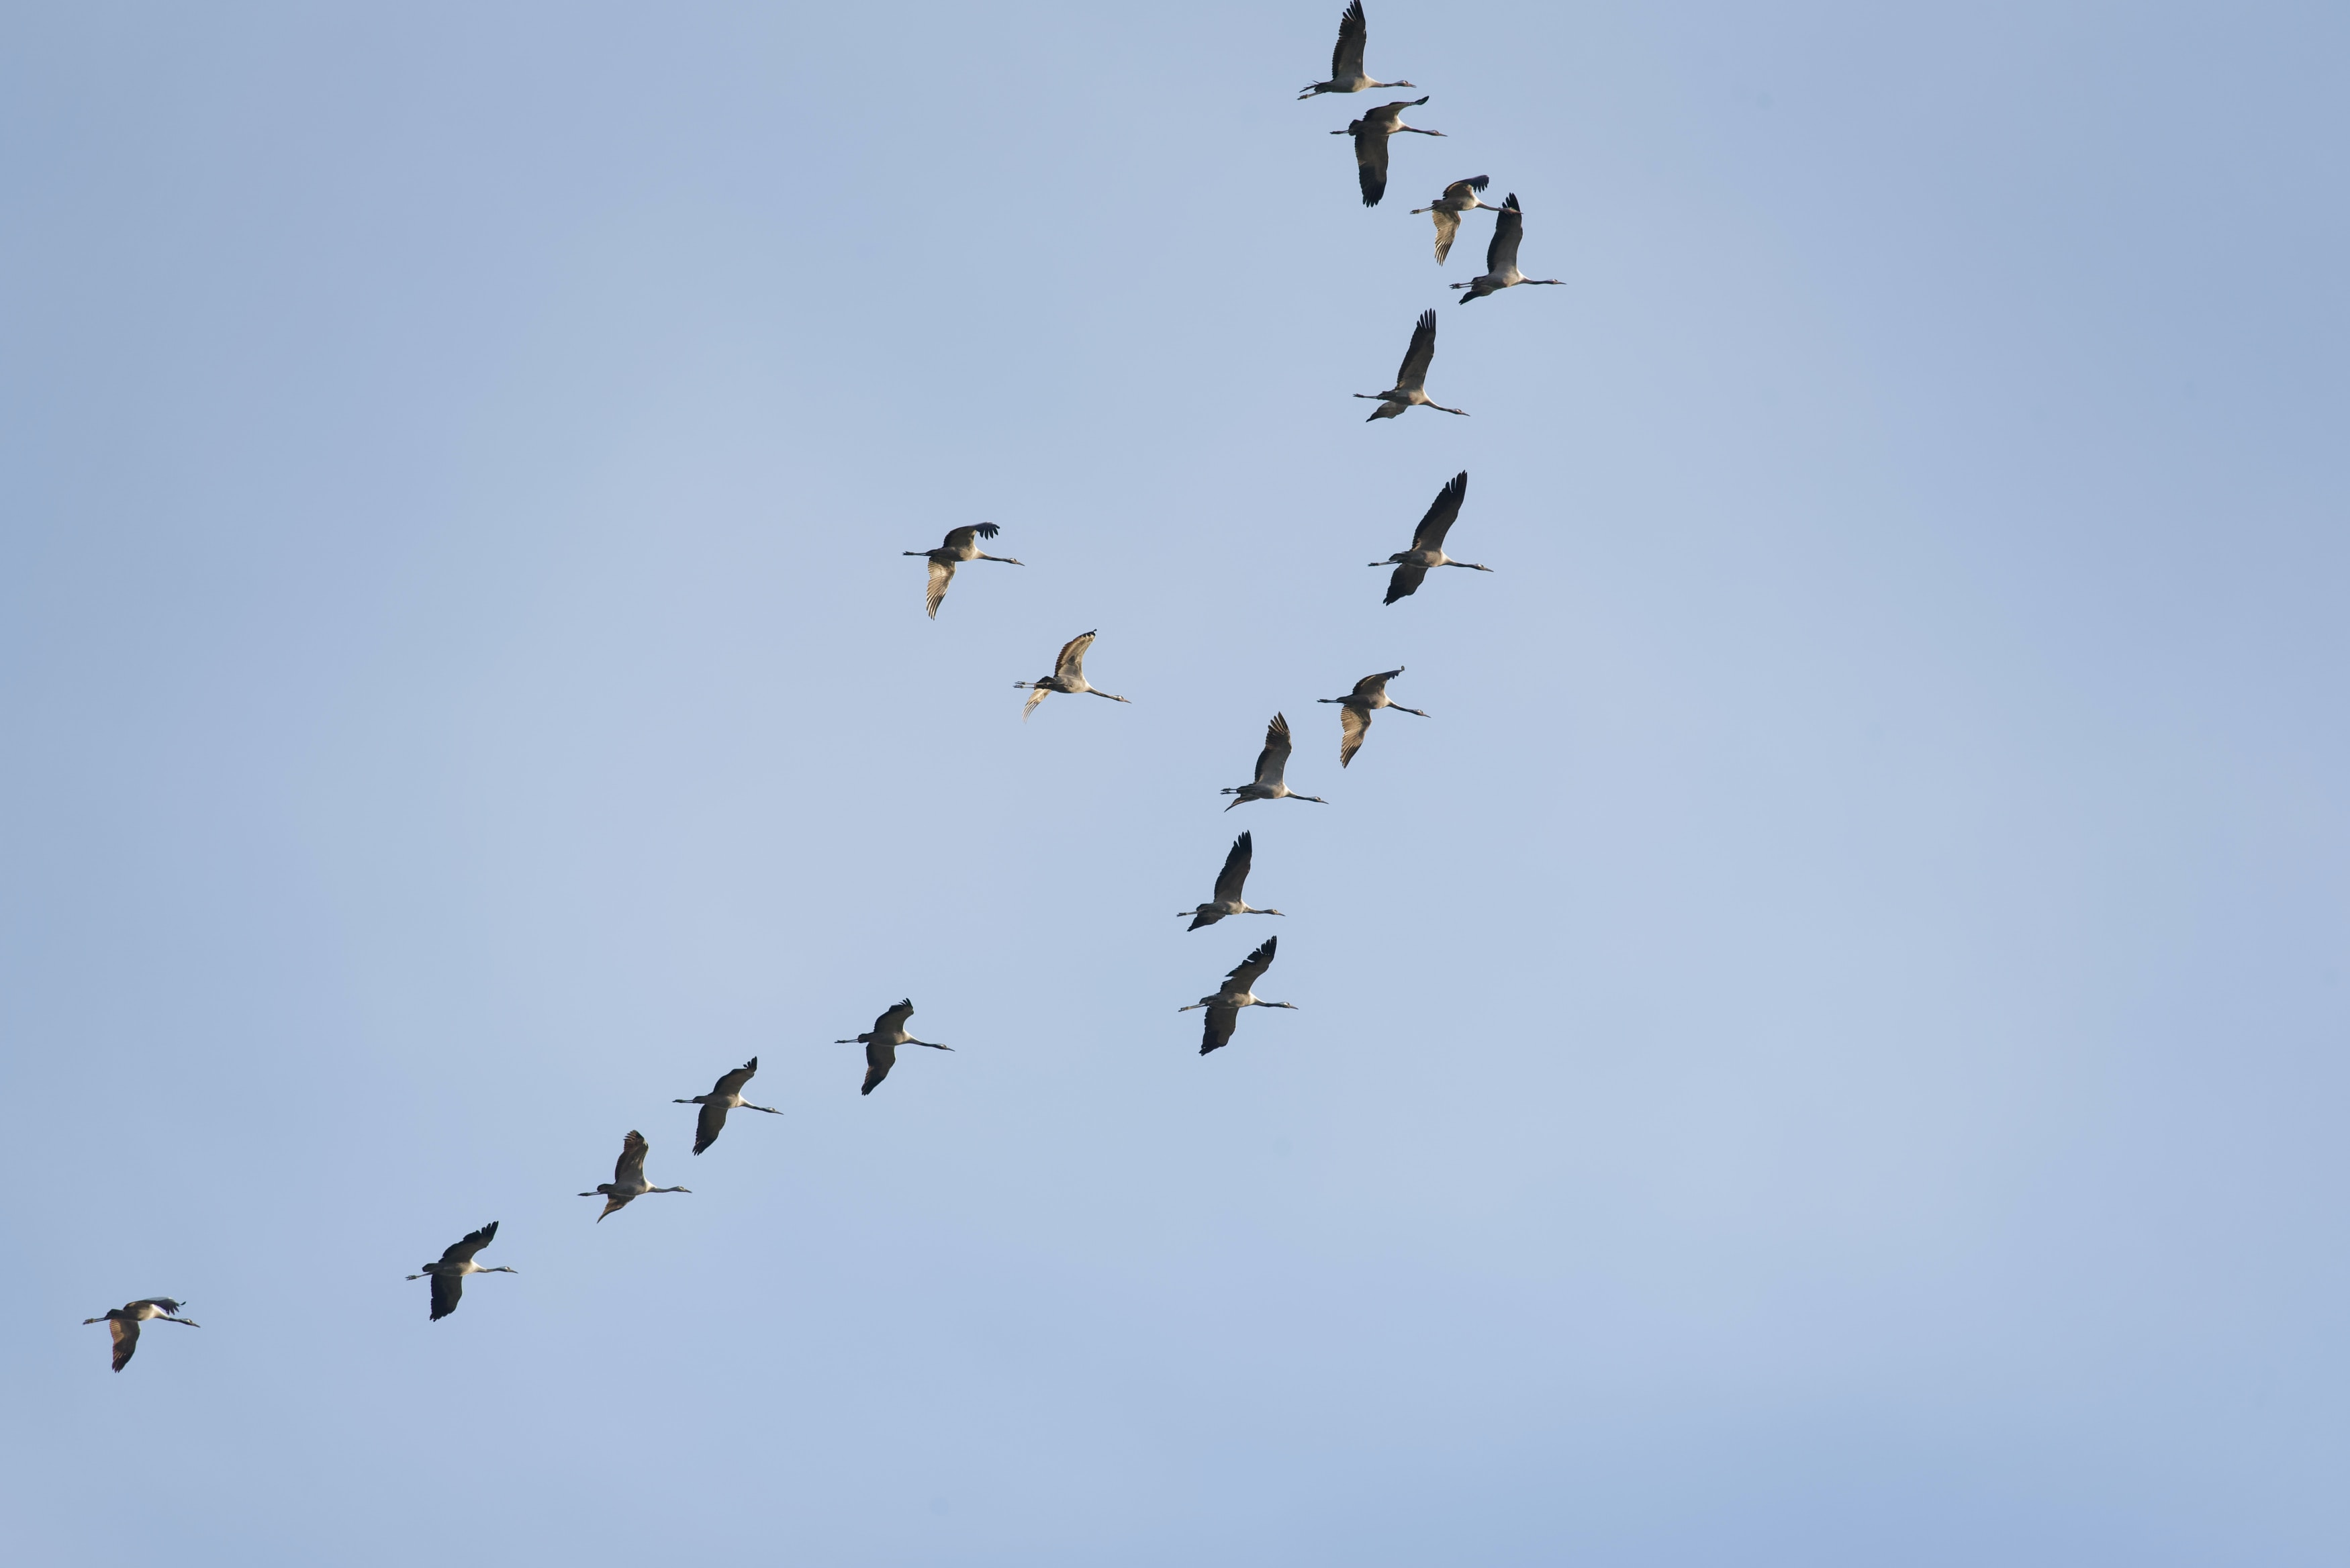
\includegraphics[scale=0.059]{plots/migrating-cranes.jpg}
        \caption{Migrating cranes (Photo by REGINE THOLEN on Unsplash)}
    \end{subfigure}
    \hfill
    \begin{subfigure}[t]{0.45\textwidth}
        \centering
        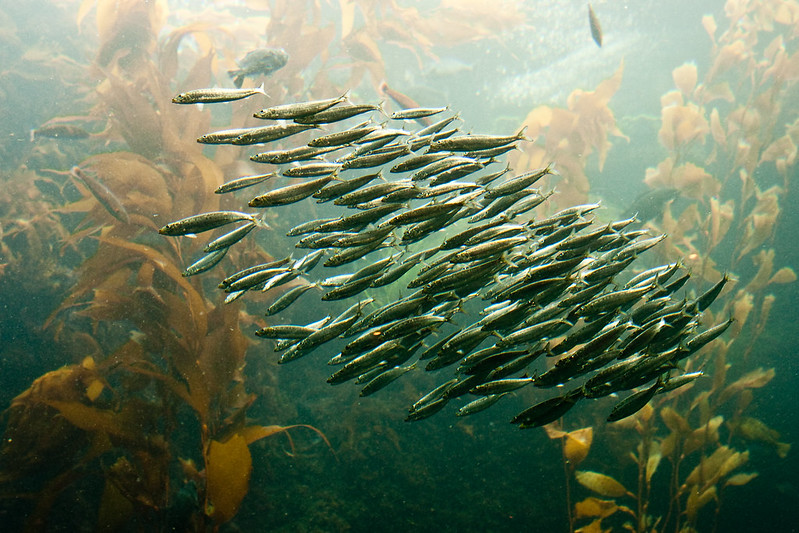
\includegraphics[scale=0.26]{plots/school-of-fish.jpg}
        \caption{School of fish (Creative commons license, Flickr)}
    \end{subfigure}
    \caption{Examples of flocking behavior in nature}
    \label{fig:intro}
\end{figure}
